\section{Aufnahmen der Sensitized Emission}
Um die Effizienz von FRET in unserer Probe zu bestimmen, haben wir verschiedene fluoreszenzmikroskopische Aufnahmen gemacht.
Zuerst wird die Hauptprobe mit sowohl CFP- als auch YPF-markierten Zellen untersucht.
Danach werden Proben, mit je nur CFP- oder YPF-Markierungen untersucht.
Diese je einmal mit Licht der Wellenlänge $458\,\text{nm}$ beleuchtet und dann die Fluoreszenz im Bereich $470-500\,\text{nm}$ (D) und $520-550\,\text{nm}$ (S) detektiert.
Danach wird die Probe nochmal mit Licht der Wellenlänge $514\,\text{nm}$ beleuchtet und die Fluoreszenz im Bereich $470-500\,\text{nm}$ gemessen.
Dabei wird noch eine Bright-Field Aufnahme gemacht.\\
Die einzelnen Bilder werden wie folgt benannt:
\begin{table}[h]
    \centering\begin{tabular}{c|ccc}
        Zelle & D & S & A\\
        \hline
        C+Y & D$_\text{CY}$ & S$_\text{CY}$ & A$_\text{CY}$\\
        C & D$_\text{CFP}$ & S$_\text{CFP}$ & A$_\text{CFP}$\\
        Y & D$_\text{YFP}$ & S$_\text{YFP}$ & A$_\text{YFP}$
    \end{tabular}
    \caption{Benennung der Aufnahmen der Sensitized Emission}
\end{table}
\subsection{Korrekturfaktoren}
Aufgrund des 'Crosstalks' (Überlappung der Anregungs- und Detektionsbereiche von Donor und Akzeptor) kann die FRET-Intensität nicht direkt gemessen werden.
Um dies zu herauszurechnen, werden bei jeweils nur CFP- und YFP-markierten Zellen die Donor-, Sensitized Emission- und Akzeptor-Intensität gemessen und folgende Korrekturfaktoren berechnet:
\begin{align}
    \alpha&=D_\text{YFP}/A_\text{YFP}\\
    \beta&=S_\text{CFP}/A_\text{CFP}\\
    \gamma&=S_\text{YFP}/A_\text{YFP}\\
    \delta&=D_\text{YFP}/A_\text{YFP}
\end{align}
Hierbei steht die Intensität für die mittlere Intensität aller Zellen.\\
Um diese zu bestimmen, wird jeweils eine Fotoserie (Donor-, Sensitized Emission-, Akzeptoremission und Brightfield) in das Programm Fiji/ImageJ geladen.
Dort wird zuerst eine ROI (region of interest) um einen zellenfreien Teil in der Brightfield Aufnahme gemalt.
Diese wird mithilfe des ROI-Managers in alle anderen Bilder kopiert und dort die mittlere Intensität gemessen.
Im nächsten Schritt wird eine zweite ROI um den fluoreszierenden Teil der Zelle gezogen und wieder auf alle Zellen kopiert.
Dort wird wieder die mittlere Intensität der Zelle gemessen.\newpage
Folgendermaßen sehen die ROIs aus:
\begin{figure}[h]
    \centering\subfigure[Zellmessung]{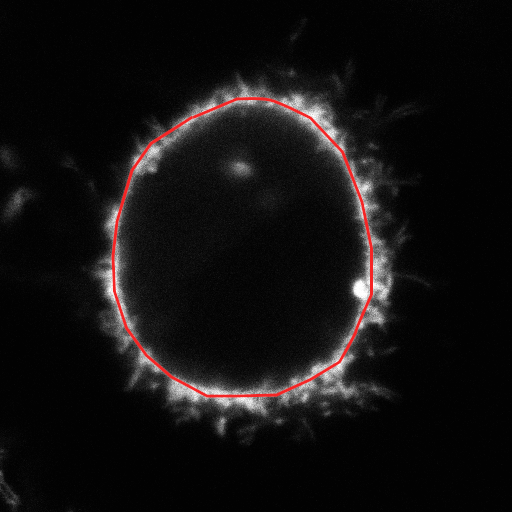
\includegraphics[width=0.2\textwidth]{Auswertung-Dominik/04-YFP-ROI.png}}
    \subfigure[Hintergrundmessung]{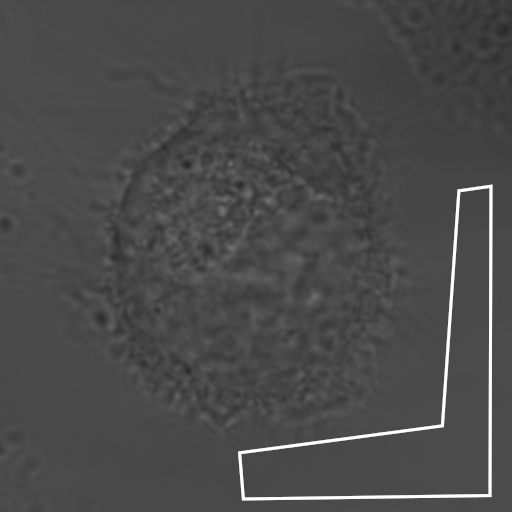
\includegraphics[width=0.2\textwidth]{Auswertung-Dominik/04-BF-ROI.png}}
    \caption{Verschiedene ROIs}
\end{figure}\\
Um nun die Korrekturfaktoren zu berechnen, wird von der Zellmessung zuerst die Hintergrundmessung abgezogen.
Danach wird für jede Zelle einzeln der Korrekturfaktor bestimmt und abschließend über alle gemittelt.\\
Somit ergeben sich folgende Korrekturfaktoren:
\begin{align*}
    \alpha&=0,030\\
    \beta&=0,207\\
    \gamma&=0,562\\
    \delta&=0,054
\end{align*}
Eine Tabelle mit allen Messungen findet sich im Anhang.
\subsection{SE und FRET Effizienz}
Zuerst werden wieder die Bilder in Fiji/ImageJ importiert.
Im nächsten Schritt wird eine ROI um einen zellenfreien Teil in der Bright Field Aufnahme eingezeichnet.
Danach wird diese, durch den ROI-Manager, auf die anderen Bilder übertragen.
Im jeweiligen Bild misst man dann die mittlere Intensität und wählt danach die ROI wieder ab.
Anschließend wird das Bild in ein 32-Bit Bild umgewandelt. Dies wird gemacht, da bei 8-Bit nur $2^8=255$ Werte für die Intensität zur Verfügung stehen.
Bei 32-Bit stehen $2^{32}\approx4,3\cdot10^9$ Werte zur Verfügung, was die Rechnungen etwas genauer macht.
Wenn das Bild umgewandelt wird, wird von dem ganzen Bild die Hintergrundmessung abgezogen.
Danach wird der 'Threshold' auf etwa 3 angehoben, was dazu führt, dass alle Pixel die einen geringeren Wert als 3 haben zu 'NaN' (NotaNumber) werden und in späteren Berechnungen nicht mehr beachtet werden.
Dies wird mit allen 3 Bildern (Donor, Sensitized Emission und Akzeptor) gemacht.
\subsubsection{Werte}
Um nun einen Zahlenwert für die Sensitized Emission zu bekommen, wird eine ROI um die einzelnen Zellen gezogen und die mittlere Intensität berechnet.
Diese wird dann mit den Korrekturfaktoren wie folgt verrechnet:
\begin{equation}
    SE=\frac{\text{S}_\text{CY}-\beta\cdot\text{D}_\text{CY}-\left(\gamma-\alpha\cdot\beta\right)\cdot\text{A}_\text{CY}}{1-\beta\cdot\delta}
\end{equation}
Die FRET-Effizienz wird danach wie folgt berechnet:
\begin{equation}
    E=\frac{SE}{\sqrt{\text{A}_\text{CY}\cdot\text{D}_\text{CY}}}
\end{equation}\newpage
Somit bekommt man folgende Wertetabelle:
\begin{table}[htbp]
    \centering
      \begin{tabular}{c|cc}
        Zelle & Sensitized Emission & FRET Intensität\\\hline
      1 & 5,1869189 & 0,49342845 \\
      2 & 13,0835367 & 0,42973668 \\
      3 & 12,0800542 & 0,96251588 \\
      4 & 15,4703842 & 0,54063115 \\
      5 & 10,3858137 & 0,50313880 \\
      6 & 28,9868398 & 0,64137183 \\
      7 & 16,5871733 & 0,84110296 \\
      8 & 26,5717226 & 0,98273363 \\
      9 & 10,5669283 & 0,65557684 \\
      10 & 9,9482744 & 0,62637984 \\
      11 & 62,5234049 & 0,63674985 \\
      12 & 12,6206028 & 0,79515135 \\
      13 & 21,7648752 & 0,65874651 \\
      14 & 21,4772655 & 0,40308614 \\
      15 & 22,0766976 & 0,69485260 \\
      16 & 23,1496922 & 0,66020480 \\
      17 & 13,8373739 & 0,63248513 \\
      18 & 7,86244379 & 0,62679721 \\
      19 & 9,15395144 & 0,62775177 \\
      20 & 9,95348719 & 0,42750202 \\
      21 & 7,38539461 & 0,48594412 \\
      \end{tabular}
    \caption{Wertetabelle Sensitized Emission und FRET-Effizienz}
    \label{tab:SE Effizienz}
  \end{table}\\
  Die einzelnen Werte für den Donor, Sensitized Emission und Akzeptor Channel findet man im Anhang.
Als Mittelwert für die Sensitized-Emission und der FRET-Effizienz folgt:
\begin{align}
  SE&=\left(17,1\pm12,0\right) & E&=\left(0,63\pm0,16\right)
\end{align}\newpage
\subsubsection{Bilder}
Um die Sensitized Emission/FRET-Effizienz auch bildlich darzustellen, kann die Gleichung der Sensitized Emission und der FRET-Effizienz auch in Fiji/ImageJ direkt umgesetzt werden.
Hierfür wird anstatt der mittleren Intensität des Donor-, bzw. Sensitized Emission- oder Akzeptor-Channel das jeweilige Bild verwendet.
Anschließend wird das Bild noch mit einer Color-Map versehen (wir haben uns für 'Green Fire Blue' entschieden), eine Legende (Calibration Bar) und Größenangabe (Scale Bar) hinzugefügt.
Somit entstehen folgende Bilder, wo man anhand der Verfärbung die FRET-Effizienz für jeden Teil der Zelle sehen kann:
\begin{figure}[h]
    \centering\subfigure[Sensitized Emission]{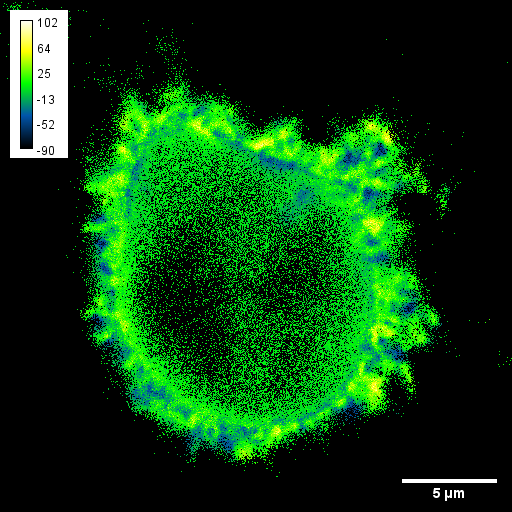
\includegraphics[width=0.3\textwidth]{Auswertung-Dominik/07-SE.png}}
    \subfigure[FRET-Effizienz]{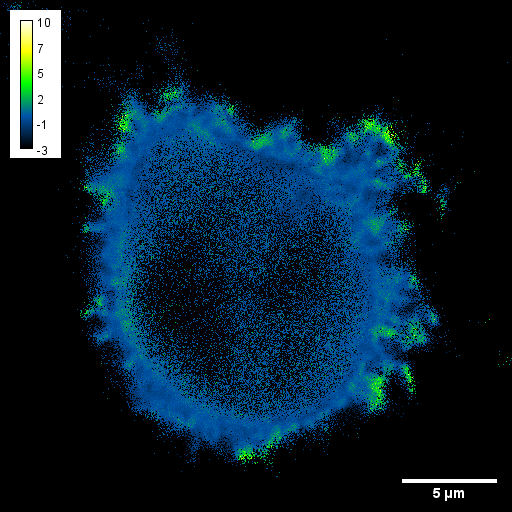
\includegraphics[width=0.3\textwidth]{Auswertung-Dominik/07-FRET.png}}
    \caption{SE und E der Zelle 7}
\end{figure}\\
Alle Bilder der Sensitized Emission und FRET-Effizienz findet man im Anhang.
\subsection{Abstand der Fluorophore}
In den Fragen zur Vorbereitung wird bei der Effizienz des FRET-Effekts folgende Formel behandelt:
\begin{equation}
    E=\frac{R_F^6}{R_F^6+R^6}
\end{equation}
Diese verknüpft die FRET-Effizienz mit dem Abstand der Proteine.
Diese Formel kann umgeschrieben werden, um den Abstand bei bekannter FRET-Effizienz zu bekommen:
\begin{align}
    E&=\frac{R_F^6}{R_F^6+R^6}\\
    \left(R_F^6+R^6\right)\cdot E&=R_F^6\\
    R&=\sqrt[6]{\frac{R_F^6}{E}-R_F^6}
\end{align}
Der ausgerechnete Wert, kann als mittlerer Abstand zwischen den Proteinen in der betrachteten Zelle interpretiert werden.\newpage
Für die einzelnen Zellen folgt, mit einem Försterradius von $4,9\,\text{nm}$ \citep[vgl.][]{foersterradius}, für den mittleren Abstand:
\begin{table}[htbp]
    \centering
      \begin{tabular}{c|c}
        Zelle & Mittlere Abstand (nm)\\\hline
      1 & 4,92151539 \\
      2 & 1,3661913 \\
      3 & 0,75876261 \\
      4 & 1,26836065 \\
      5 & 1,30054053 \\
      6 & 1,18291925 \\
      7 & 0,98721207 \\
      8 & 0,66449782 \\
      9 & 1,17069601 \\
      10 & 1,19572534 \\
      11 & 1,18687643 \\
      12 & 1,03959272 \\
      13 & 1,16795419 \\
      14 & 1,39139887 \\
      15 & 1,13623678 \\
      16 & 1,1666908 \\
      17 & 1,19052023 \\
      18 & 1,19536991 \\
      19 & 1,19455678 \\
      20 & 1,36827055 \\
      21 & 1,31553785 \\
      \end{tabular}
    \label{Mittlere Abstand der Proteine in den Zellen}
  \end{table}\\
Wenn man nun dies noch über alle Zellen mittelt, erhält man, dass in allen Probe im Mittel der Abstand der Proteine $\left(1,3\pm0,8\right)\,\text{nm}$ beträgt.